\chapter{Resultados}
\label{resultados}

Neste capítulo apresentaremos os espectros de massa referentes aos \textit{clusters} de prata, que caracterizam os resultados experimentais obtidos neste trabalho.

\section{Espectros de nanopartículas de prata}
\label{sec:producao_cluster}
Foram realizados quatro experimentos para obtenção dos espectros de prata. Para cada um foram obtidos os dados dos \textit{clusters} com e sem a incidência de luz ultra violeta. 

Os dados fornecidos pelo sistema de aquisição
fornece o tempo de voo das partículas e as intensidade dos picos, como pode ser visto na Figura \ref{fig:ex_dados_brutos}. Depois de adquirido, os dados são tratados de forma a minimizar os ruídos existentes, e é feita uma normalização pela eficiência do detector de corrente, uma vez que as partículas com menor massa são melhor detectadas do que as partículas de maiores massas. O mesmo espectro com o tratamento de dados realizado pode ser visto na \ref{fig:0105_ledoff_dados_tratados}.




\begin{figure}
  \centering  
  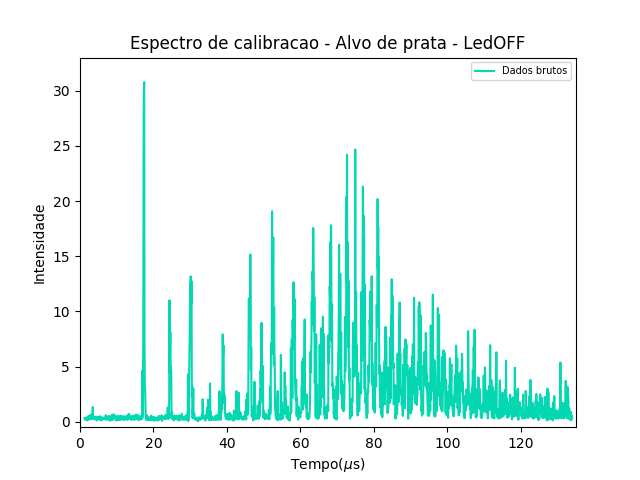
\includegraphics[width=0.7\textwidth]{exp_01/LedOFF_sem_tratamento.png}
  \caption{Espectro de calibração sem tratamento de dados.}
  \label{fig:ex_dados_brutos} 
\end{figure}

\begin{figure}
  \centering  
  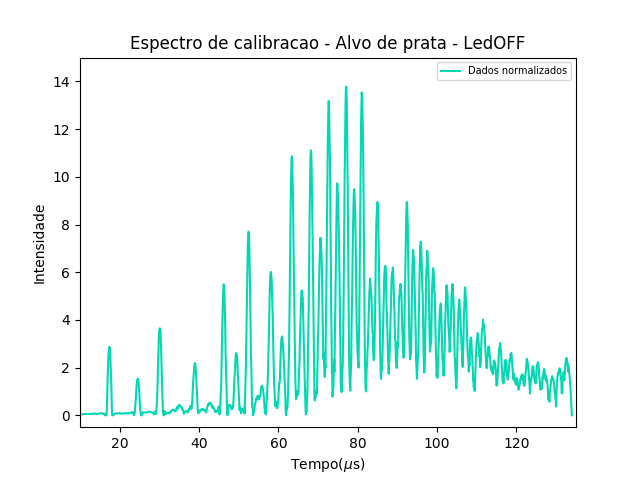
\includegraphics[width=0.7\textwidth]{exp_01/LedOFF_normalizado_mcp.png}
  \caption{Espectro de calibração com tratamento de dados.}
  \label{fig:0105_ledoff_dados_tratados} 
\end{figure}

Para indicar quais são os picos presentes nos espectros, e assim encontrar as indicações do número de prata ($Ag_{1},Ag_{2},Ag_{3}...$), é necessário realizar uma calibração, \textcolor{blue}{onde são relacionadas o tempo de voo de cada partícula com o quociente massas/carga, como explicitado na Equação \ref{eq:tempo_voo}}, de forma a obter uma tendência quadrática, como veremos a seguir.

Com o objetivo de obter uma maior precisão na determinação dos tempos de voo das partículas de prata, é traçado uma curva gaussiana em cima de cada pico do espectro. \textcolor{blue}{A gaussiana traçada possui uma largura de $2\mu$ segundos, fato esse que será utilizado para encontrar as incertezas dos dados obtidos.}

A Tabela \ref{tab:picos_encontados_01} mostra os valores dos picos encontrados, em comparação com os valores dos picos calculados teoricamente pela Equação \ref{eq:relacao_massa_tempo}. \textcolor{blue}{ Note que os resultados obtidos encontram-se dentro da margem de incerteza, implicando que os picos encontrados correspondem com os que eram esperados.} 

\begin{table}
\centering
\caption{I- Tempo de voo dos átomos de Prata}
\label{tab:picos_encontados_01}
\begin{tabular}{|c|c|c|c|c|c|c|}
\hline
\begin{tabular}[c]{@{}c@{}}Prata\\ (N)\end{tabular} & \begin{tabular}[c]{@{}c@{}}Massa\\ teórica\\ (u.m.a)\end{tabular} & \begin{tabular}[c]{@{}c@{}}LED OFF\\ Massa\\ calculada\\ $\pm \Delta m$\\ (u.m.a)\end{tabular} & \begin{tabular}[c]{@{}c@{}}LED ON\\ Massa\\ calculada\\ $\pm \Delta m$\\ (u.m.a)\end{tabular} & \begin{tabular}[c]{@{}c@{}}Tempo\\ teórico\\ ($\mu s$)\end{tabular} & \begin{tabular}[c]{@{}c@{}}LED OFF\\ Tempo\\ calculado\\ $\pm \Delta t$\\ ($\mu s$)\end{tabular} & \begin{tabular}[c]{@{}c@{}}LED ON\\ Tempo\\ calculado\\ $\pm \Delta t$\\ ($\mu s$)\end{tabular} \\ \hline 
1&107.86&104$\pm$25&106$\pm$26&17.30&17$\pm$2&17$\pm$2\\ \hline 
2&215.72&215$\pm$35&215$\pm$35&24.47&24$\pm$2&24$\pm$2\\ \hline 
3&323.58&322$\pm$42&324$\pm$42&29.96&30$\pm$2&30$\pm$2\\ \hline 
4&431.44&438$\pm$49&433$\pm$48&34.60&35$\pm$2&34$\pm$2\\ \hline 
5&539.30&536$\pm$54&538$\pm$54&38.68&38$\pm$2&38$\pm$2\\ \hline 
6&647.16&652$\pm$59&650$\pm$59&42.38&42$\pm$2&42$\pm$2\\ \hline 
7&755.02&756$\pm$64&756$\pm$63&45.77&46$\pm$2&46$\pm$2\\ \hline 
8&862.88&857$\pm$68&859$\pm$68&48.93&49$\pm$2&49$\pm$2\\ \hline 
9&970.74&966$\pm$72&968$\pm$72&51.90&52$\pm$2&52$\pm$2\\ \hline 
10&1078.60&1092$\pm$76&1087$\pm$76&54.71&55$\pm$2&55$\pm$2\\ \hline 
11&1186.46&1179$\pm$79&1180$\pm$79&57.38&58$\pm$2&58$\pm$2\\ \hline 
12&1294.32&1293$\pm$83&1291$\pm$83&59.93&60$\pm$2&60$\pm$2\\ \hline 
13&1402.18&1399$\pm$86&1400$\pm$86&62.38&63$\pm$2&63$\pm$2\\ \hline 
14&1510.04&1512$\pm$90&1509$\pm$89&64.73&65$\pm$2&65$\pm$2\\ \hline 
15&1617.90&1614$\pm$93&1618$\pm$92&67.00&68$\pm$2&68$\pm$2\\ \hline 
16&1725.76&1720$\pm$95&1728$\pm$95&69.20&70$\pm$2&70$\pm$2\\ \hline 
17&1833.62&1829$\pm$98&1833$\pm$98&71.33&72$\pm$2&72$\pm$2\\ \hline 
18&1941.48&1938$\pm$101&1941$\pm$101&73.40&74$\pm$2&74$\pm$2\\ \hline 
19&2049.34&2053$\pm$104&2048$\pm$104&75.41&77$\pm$2&76$\pm$2\\ \hline 
20&2157.20&2164$\pm$107&2158$\pm$107&77.37&79$\pm$2&79$\pm$2\\ \hline 
\end{tabular} 
\end{table} 


Sabendo o número de átomos de prata que corresponde a cada tempo de voo, é possível plotar uma curva de calibração, \textcolor{blue}{massa (em função da carga) $\times$ tempo}, e assim realizar uma ajuste de uma curva quadrática, onde os coeficientes que vão permitir identificar a massa de todo o espectro adquirido, seguindo a equação \ref{eq:0105_polinomio_calib_ledoff}. O ajuste do espectro em questão pode ser vista na Figura \ref{fig:1105_curva_calib_ledoff}.

\begin{equation}
\label{eq:0105_polinomio_calib_ledoff}
M(t) = 0,3304t^2 + 1,445t - 20,2
\end{equation}
\begin{figure}
  \centering  
  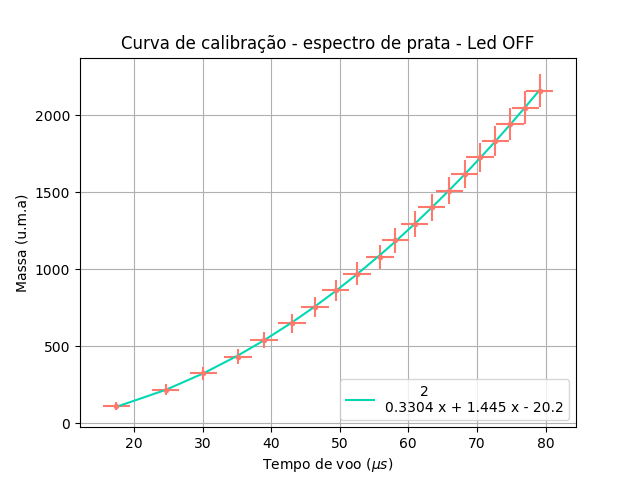
\includegraphics[width=0.7\textwidth]{exp_01/LEDOFF_curv+erro_calib.png}
  \caption{Curva de calibração.}
  \label{fig:1105_curva_calib_ledoff} 
\end{figure}



\textcolor{red}{Precisa explicar que é massa/carga}







Os erros foram calculados a partir da Equação \ref{eq:0105_polinomio_calib_ledoff}, da seguinte forma:

\begin{equation}
    \Delta M(t) = \frac{\partial M(t)}{\partial t} \times \Delta t
\end{equation}
onde $\Delta t = 2 \mu $ segundos.

E então para este caso, a equação para o cálculo do erro é dada por:

\begin{equation}
    \Delta M(t) = (2\times 0,3304 \times t + 1,445) \times 2
\end{equation}


Utilizando a Equação \ref{eq:0105_polinomio_calib_ledoff} é possível mudar o eixo de tempo de voo, da aquisição de dados, para o seu valor corresponde em massa, conforme do gráfico da Figura \ref{fig:0105_LEDOFF_espec_calib_ag_massa}.



\begin{figure}
  \centering  
  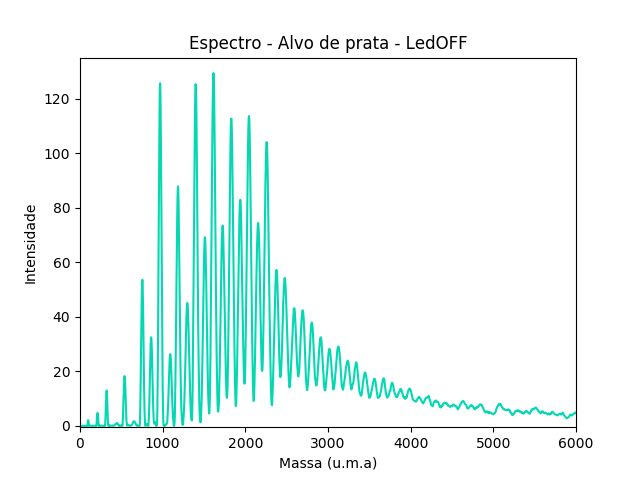
\includegraphics[width=0.7\textwidth]{graficos_resultados/0105_LEDOFF_espec_calib_ag_massa}
  \caption{Espectro de prata plotado na forma de intensidade por massa em unidade de massa atômica.}
  \label{fig:0105_LEDOFF_espec_calib_ag_massa} 
\end{figure}

Com o espectro em função da massa das \textit{clusters}, é possível identificar as partículas de prata com: um, dois, três... \textit{n} átomos, conforme mostra o gráfico da Figura \ref{fig:exp_01_LEDONOFF_N}. O gráfico apresenta também a relação entre os espectros com o LED ligado e desligado. Para obter a curva "\textit{LED ON}", foi utilizado o mesmo procedimento descrito anteriormente para a curva "\textit{LED OFF}".

Os espectros referentes ao dados com a incidência de luz ultra violeta, assim como a curva de calibração, serão apresentados no Apêndice \ref{sec:apendice}.

\begin{figure}
  \centering  
  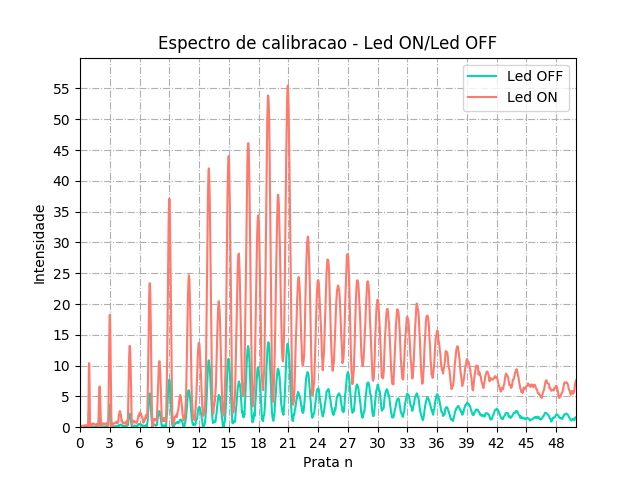
\includegraphics[width=0.7\textwidth]{exp_01/Led_ON_Led_OFF_espectro_calib_prata_N_}
  \caption{I-Espectro de prata, com LED ligado e desligado, na forma de intensidade por massa em unidade de massa atômica.}
  \label{fig:exp_01_LEDONOFF_N}
\end{figure}

Para obter uma boa estatística, foram realizados mais três experimentos os quais os espectro de prata, com LED ligado e desligado, na forma de intensidade por massa em unidade de massa atômica, podem ser vistos nas Figuras \ref{fig:exp_02_LEDONOFF_N}, \ref{fig:exp_03_LEDONOFF_N} e \ref{fig:exp_04_LEDONOFF_N}. As curvas de calibração, e as tabelas utilizadas para conversão serão apresentadas na \ref{sec:apendice}

\begin{figure}
  \centering  
  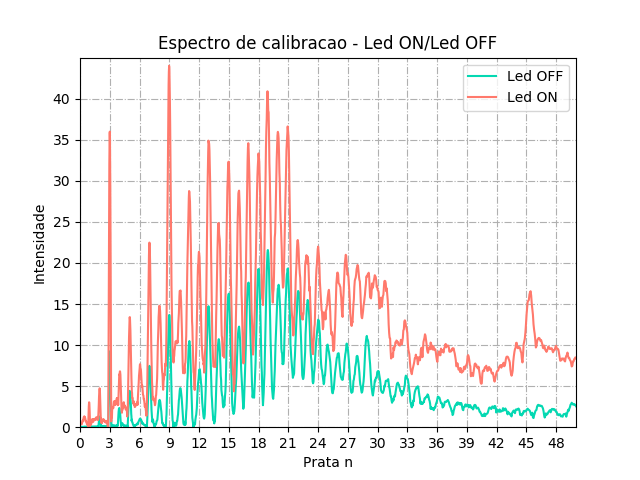
\includegraphics[width=0.7\textwidth]{exp_02/LED_ON_Led_OFF_espectro_calib_prata_N_.png}
  \caption{II- Espectro de prata, com LED ligado e desligado, na forma de intensidade por massa em unidade de massa atômica.}
  \label{fig:exp_02_LEDONOFF_N}
\end{figure}

\begin{figure}
  \centering  
  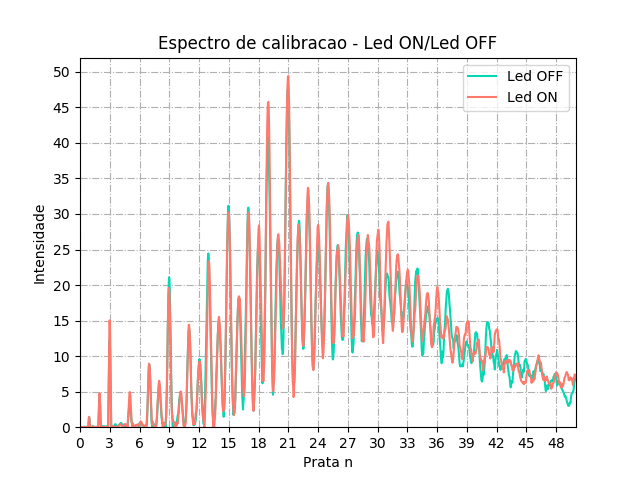
\includegraphics[width=0.7\textwidth]{exp_03/LED_ON_Led_OFF_espectro_calib_prata_N_.png}
  \caption{III-Espectro de prata, com LED ligado e desligado, na forma de intensidade por massa em unidade de massa atômica.}
  \label{fig:exp_03_LEDONOFF_N}
\end{figure}

\begin{figure}
  \centering  
  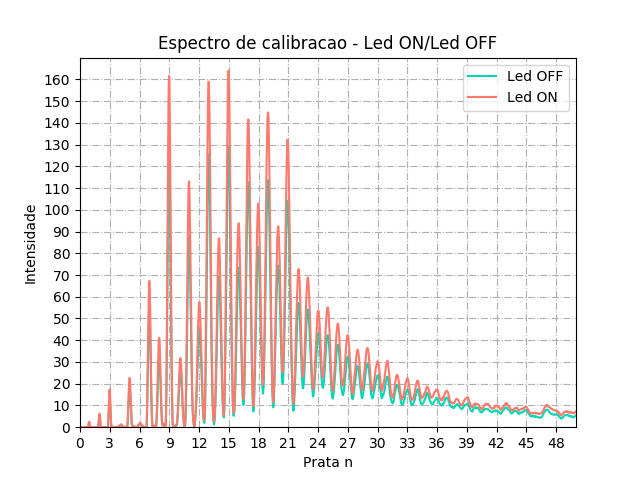
\includegraphics[width=0.7\textwidth]{exp_04/LED_ON_Led_OFF_espectro_calib_prata_N_.png}
  \caption{IV-Espectro de prata, com LED ligado e desligado, na forma de intensidade por massa em unidade de massa atômica.}
  \label{fig:exp_04_LEDONOFF_N}
\end{figure}

Note que nos resultados apresentados foi obtido o mesmo comportamento do experimento realizado por Katakuse et al \cite{KATAKUSE1985229}, em 1985 com, partícula de prata, já citado na secção \ref{sec:experimentos_teo}. Foram encontrados padrões com picos bem definidos em cada um espectro de massa e podemos apontar uma maior  abundância nos picos como número de átomos iguais, $n= 3,9,21,35...$. Esses picos ocorrem devido ao preenchimento das camadas eletrônicas, pelo princípio de exclusão de Pauli.

 No nosso caso as partículas de prata produzidas são carregada negativamente, ou seja, possuem um elétrons a mais, dessa forma temos que:
  \begin{equation*}
    Ag_{2} \to Ag_{2} + e^{-}
\end{equation*} 
 Fato esse que resulta nos "números mágicos" iguais à $n= 3,9,21,35...$. Além disso podemos notar que existe uma maior abundância dos \textit{clusters} com números ímpares de átomos em relação ao \textit{clusters} com números pares de átomos, isso também se deve a estabilidade dessas partículas.
 
 Fato que também podemos notar observando os espectros de partículas de prata apresentados nas Figuras \ref{fig:exp_01_LEDONOFF_N}, \ref{fig:exp_02_LEDONOFF_N} e \ref{fig:exp_04_LEDONOFF_N}, é que a intensidade dos picos, quando o LED encontra-se ligado, é superior a intensidade dos picos quando o LED encontra-se desligado. Isso ocorre devido ao fato da incidência de luz ultravioleta ioniza ainda mais as partículas que partem do \text{sputtering}, assim grande parte das partículas que antes eram neutras e eram barradas pelas lentes eletrostáticas agora são ionizadas e conseguem atingir a amostra, aumentando a intensidade da corrente medida.
 
 Os gráficos das Figuras \ref{fig:exp_01_picos_LEDONOFF_N}, \ref{fig:exp_02_picos_LEDONOFF_N} e \ref{fig:exp_04_picos_LEDONOFF_N} mostram mais explicitamente o fato citado.
 
 
 \begin{figure}
  \centering  
  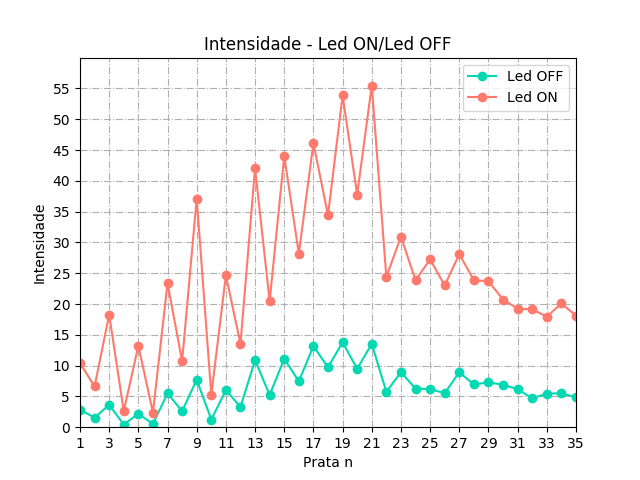
\includegraphics[width=0.7\textwidth]{exp_01/Led_ON_Led_OFF_intensidade_prata_N_.png}
  \caption{I - Relação de intensidade dos picos de prata, com LED ligado e desligado, na forma de intensidade por massa em unidade de massa atômica.}
  \label{fig:exp_01_picos_LEDONOFF_N}
\end{figure}
 
 \begin{figure}
  \centering  
  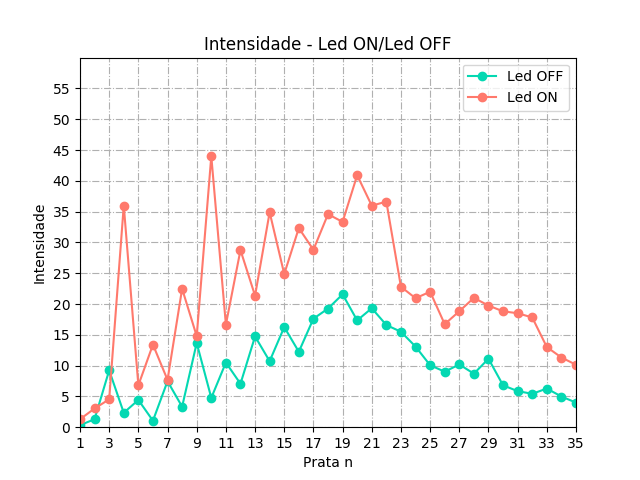
\includegraphics[width=0.7\textwidth]{exp_02/LED_ON_Led_OFF_intensidade_prata_N_.png}
  \caption{II - Relação de intensidade dos picos de prata, com LED ligado e desligado, na forma de intensidade por massa em unidade de massa atômica.}
  \label{fig:exp_02_picos_LEDONOFF_N}
\end{figure}
 
  \begin{figure}
  \centering  
  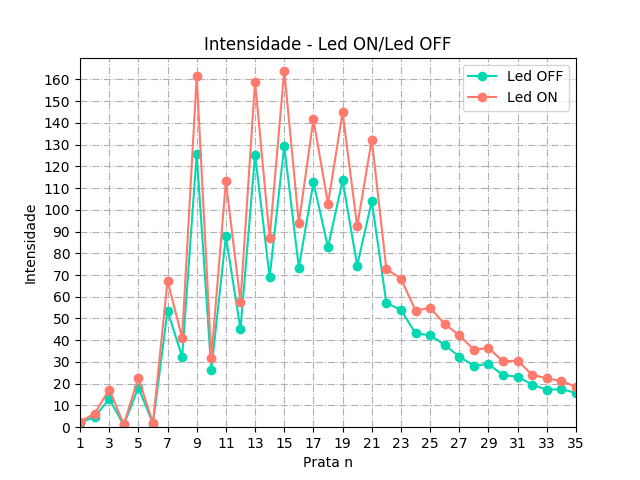
\includegraphics[width=0.7\textwidth]{exp_04/LED_ON_Led_OFF_intensidade_prata_N_.png}
  \caption{IV - Relação de intensidade dos picos de prata, com LED ligado e desligado, na forma de intensidade por massa em unidade de massa atômica.}
  \label{fig:exp_04_picos_LEDONOFF_N}
\end{figure}

Fato esse que não fica evidente no gráfico apresentado na Figura \ref{fig:exp_03_picos_LEDONOFF_N}, uma vez que esse experimento foi realizado no final do tempo de vida útil do alvo de prata e a corrente costuma cair rapidamente ao longo do tempo nesta situação. O protocolo experimental era realizar primeiro as medidas com o LED desligado e depois com o LED ligado, por isso temos alguns picos com o LED desligado que possuem maior intensidade. Com o alvo limitando a corrente fornecida, não havia um número átomos suficiente para ser ionizados pela luz ultravioleta e então não é possível notar uma grande diferença de intensidade.  

\begin{figure}
  \centering  
  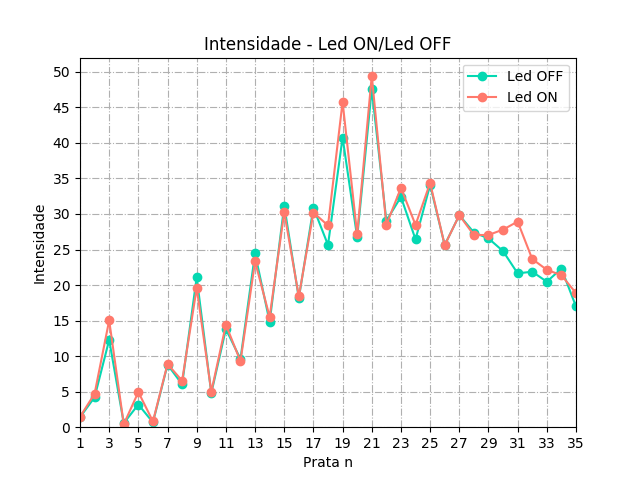
\includegraphics[width=0.7\textwidth]{exp_03/LED_ON_Led_OFF_intensidade_prata_N_.png}
  \caption{IV - Relação de intensidade dos picos de prata, com LED ligado e desligado, na forma de intensidade por massa em unidade de massa atômica.}
  \label{fig:exp_03_picos_LEDONOFF_N}
\end{figure}